\documentclass[../../main.tex]{subfiles}
\begin{document}

\subsection*{7.12}
Una spira quadrata di lato $a=20cm$ è posta nel piano xy ed è percorsa dalla corrente $i = 5A$ nel verso indicato.
\\Essa risente dell'azione del campo magnetico $\vec{B} = \alpha x \vec{u_z}$ con $\alpha = 0.2 \frac{T}{m}$.
\\Calcolare la forza F che agisce sulla spira e l'energia potenziale magnetica $U_p$.
\\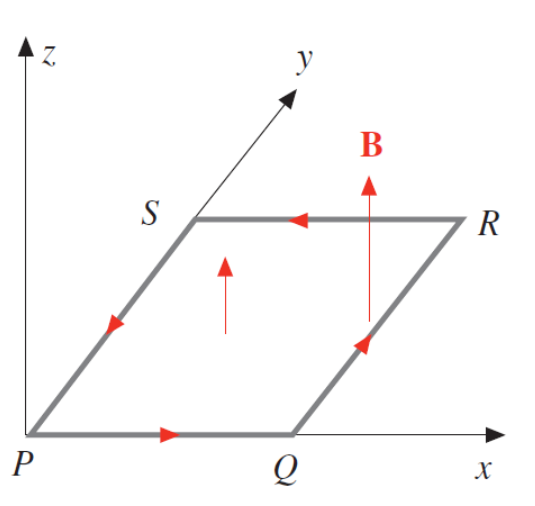
\includegraphics[scale=0.3]{e_7_12.png}
\subsubsection*{Formule utilizzate}
$\vec{F} = i\int_a^bd\vec{s}x\vec{B}$
\\$U_p = -\vec{m} * \vec{B}$
\\$ \vec{m} = i S \vec{u_n}$
\subsubsection*{Soluzione punto a}
se x = a, $\beta = \alpha a$
\\sapendo $d\vec{s}\perp \vec{B}$
\\$\vec{F_{PQ}} = \frac{i\alpha a^2}{2}$
\\$\vec{F_{QR}} = i\int_Q^Rdy\alpha a = i\alpha a[y]_Q^R = i \alpha a^2 (\vec{u_x})$
\\Sommando i quattro vettori capiamo che si annullano le due sulle y
\\Le forze su y non si annullano perchè dipendono da x, e si azzera solo quella con x = 0 perchè li il campo $  vec{B} = \alpha x $ vale 0 per x = 0.
\\$\vec{F} = \vec{F_{SP}} + \vec{F_{PQ}} + \vec{F_{QR}} + \vec{F_{RS}} = 0 - \frac{i\alpha a^2}{2}\vec{u_y} + i\alpha a^2\vec{u_x} + \frac{i\alpha a^2}{2}\vec{u_y} = i \alpha a^2 \vec{u_x}$
\subsubsection*{Soluzione punto b}
Per la regola della mano destra sappiamo che l'energia potenziale magnetica è uscente dal piano xy.
\\Però lungo la spira il campo magnetico B non è costante, quindi dobbiamo integrare per ottenere l'energia
\\$U_p = -\int_\Sigma d\vec{m} * \vec{B}$
\\$d\Sigma = adx$
\\$d\vec{m} = id\Sigma\vec{u_n} = i a dx \vec{u_n}$
\\$dU_p = iadx\vec{u_n}\vec{B} = -iadx(\vec{u_z})\alpha x \vec{u_z} = -ia\alpha x dx$
\\$U_p = -ia\alpha \int_0^axdx = -\frac{i\alpha a^3}{2}$
\newpage

\end{document}